\documentclass[11pt,a4paper]{article}

% Essential packages
\usepackage[utf8]{inputenc}
\usepackage[T1]{fontenc}
\usepackage{amsmath}
\usepackage{booktabs}
\usepackage{graphicx}
\usepackage{authblk}
\usepackage{apacite}
\usepackage{csquotes}
\usepackage{array}
\usepackage{multirow}

% Document information
\title{Bridging Ethnic Boundaries: The Evolution of Interethnic Marriages in China, 1982-2010}

% Authors and affiliations
\author[1]{Yanwen Wang}
\author[1,2]{Zheng Mu}
\affil[1]{Department of Sociology and Anthropology, National University of Singapore}
\affil[2]{Centre for Family and Population Research, National University of Singapore}

\providecommand{\keywords}[1]{\textbf{Keywords:} #1}

\begin{document}

\maketitle

\sloppy

\begin{abstract}
    In multiethnic societies, interethnic marriage serves as a critical lens for
    understanding cultural integration and status hierarchies among ethnic
    groups.
    Using data from China's Census (1982-2010), we examine how these dynamics
    unfold in a context where traditional ethnic hierarchies intersect with
    state interventions through preferential policies.
    Although uncommon, intermarriage with the Han majority gradually increased,
    occurring most frequently among the Manchu, Mongolian, and Southern
    minorities, and least frequently among the Kazakh and Uyghur.
    After controlling for ethnic compositions, all minority ethnic groups
    exhibited preferences against intermarriage with the Han, with the strongest
    disinclination observed among groups maintaining distinct ethnoreligious
    identities (e.g., Kazakh, Uyghur).
    However, these cultural boundaries became increasingly permeable over time
    for most groups except the Manchu.
    Our analysis of educational patterns reveals two distinct mechanisms for
    boundary crossing: highly assimilated groups (e.g., Hui, Manchu, Mongolian)
    through educational assortative mating, others through status
    exchange--Koreans leveraged their educational advantage to marry Han
    spouses, while Han Chinese needed higher education to marry into Tibetan and
    Southern minorities.
    These findings reveal how marriage choices embody complex negotiations
    between cultural preservation, social mobility, and state-structured
    incentives, providing insights into the persistence and malleability of
    ethnic boundaries in contemporary societies.
\end{abstract}
\keywords{Interethnic marriage, ethnicity, education, status exchange, China}

\section{Introduction}

Your introduction content goes here.


\section{Data and methods}


\subsection{Data and sample}

This study uses data from the National Population Census of China conducted in
1982, 1990, 2000, and 2010.
Census data are widely regarded as the most comprehensive source of information
on the Chinese population, providing a large sample that covers all officially
recognized ethnic groups without sampling bias.

To identify married couples within individual-level Census data, we matched
spouses residing in the same household using five relationship categories to
the household head: head and spouse, parent and parent, parent-in-law and
parent-in-law, grandparent and grandparent, and children and children-in-law.
For households with multiple potential pairs within the same category, we used
year of first marriage (when available) as the matching criterion.
Because our matching method identified each marriage from both spouses' records,
we eliminated duplicates by focusing on female respondents.

Our final sample consists of 2,488,992 married women aged 25-34 who had
complete information for both their own and their spouse's ethnicity and
education.
We selected the 25-34 age range to minimize potential biases from
further educational advancement, early marriage, remarriage, bereavement, and
overlapping cohorts across census years.
\subsection{Measures}

To balance ethnic diversity with adequate sample sizes, we followed \citeauthor{ma_ethnic_2008}'s
(\citeyear{ma_ethnic_2008}) approach of grouping 55 minority ethnicities into eight larger
categories. This classification reflects population size, geographic concentration,
linguistic and religious affiliations, historical relationships with the central
government, and international sovereignty of ethnic groups:

\begin{enumerate}
    \item Hui: Hui, Salar, Dongxiang, Baoan
    \item Kazakh: Kazakh, Uzbek, Tajik, Kyrgyz, Tatars, Russian
    \item Korean: Korean
    \item Manchu: Manchu, Hezhen, Xibe
    \item Mongolian: Mongolian, Oroqen, Ewenki, Daur
    \item Tibetan: Tibetan, Yugur, Menba (Monba), Lhoba, Tu
    \item Uyghur: Uyghur
    \item Southern minorities: Other ethnic minorities concentrating in Yunnan, Guizhou,
          and Guangxi provinces.
\end{enumerate}

We classified educational attainment into three levels: low (\textit{primary school
    or less}), middle (\textit{middle school}), and high (\textit{high school or above}).
This ensures adequate sample sizes at each educational level across ethnic groups and
census years. For our analysis of status exchange, we created a more granular measure
by converting the original educational scale from 1 (\textit{illiterate}) to 6
(\textit{BA or higher}) into gender-specific percentile ranks within 11-year moving
cohorts.

\subsection{Analytical strategy}

Log-linear models are the gold standard for analyzing marriage patterns, as they
allow us to estimate spousal associations while controlling for marginal
distributions of characteristics like ethnicity and education.
This control is particularly important because ethnic and educational
compositions of husbands and wives differ and change over time, and observed
marriage patterns are typically different from those expected under random
sorting.
Following convention, we refer to these spousal associations as assortative
mating preferences, though they reflect the causes to observed patterns
deviating from random ones rather than directly measured preferences.

We employ two sets of log-linear models.
The frist set estimates marriages by husband's and wife's ethncity (nine categories each)
across four census years (1980, 1990, 2000, and 2010), yielding 144 cells
($9 \times 9 \times 4 = 144$) after cross-tabulation.
The baseline model is specified as:

\begin{equation}
    \log F_{ijt} = \beta_0 + \beta_i^{HG} + \beta_j^{WG} + \beta_t^T + \beta_{it}^{HGT} + \beta_{jt}^{WGT}
\end{equation}

\noindent where $F_{ijt}$ is the number of marriages between husbands in ethnic
group $i$ and wives in ethnic group $j$ in year $t$,
$\beta_0$ is the constant,
$\beta_i^{HG}$ and $\beta_j^{WG}$ are husbands' and wives' ethnic groups,
respectively,
$\beta_t^T$ represents the year,
and $\beta_{it}^{HGT}$ and $\beta_{jt}^{WGT}$ denote the interactions between
year and ethnic group for husbands and wives, respectively.

In our second set of models, we incorporate educational attainment alongside
ethnicity.
These models predict the number of marriages for each combination of husband's
and wife's ethnicity and education across census years, yielding 2,916 cells
($9 \times 9 \times 3 \times 3 \times 4 = 2,916$).
The baseline model is specified as:

\begin{equation}
    \log F_{ijmnt} = \beta_0 + \beta_i^{HG} + \beta_j^{WG} + \beta_m^{HE} + \beta_n^{WE} +
    \beta_t^T + \beta_{imt}^{HGET} + \beta_{jnt}^{WGET}
\end{equation}

\noindent where $F_{ijmnt}$ is the number of marriages between husbands in
ethnic group $i$ and education group $m$ and wives in ethnic group $j$ and
education group $n$ in year $t$.
In addition to the previously defined parameters,
$\beta_m^{HE}$ and $\beta_n^{WE}$ denote husbands' and wives' education,
respectively,
and $\beta_{imt}^{HGET}$ and $\beta_{jnt}^{WGET}$ capture all two- and
three-way interactions between ethnic group, education, and year for husbands
and wives, respectively.

While log-linear models effectively disentangle assortative mating preferences
from marginal distributions, their use in analyzing status exchange within
minority-majority intermarriages has notable limitations:
they are complex, subject to controversial specifications and interpretations,
and unable to capture detailed status differentiation \cite{xie_new_2021}.
To address these limitations, we employ the Exchange Index,
a model-free approach proposed by \citeauthor{xie_new_2021}
\citeyear{xie_new_2021} that offers straightforward and unambiguous
interpretation.

The Exchange Index computation involves three essential steps for each
gender-specific ethnic pairing:

\begin{enumerate}
    \item Converting educational attainment into percentile ranks within gender
          and 11-year moving cohorts,
    \item Performing full exact matching between treated (interethnic marriage)
          and control (intra-ethnic marriage) cases, based on husbands'
          educational percentile and age, then wives',
    \item Estimating the difference in spousal educational percentiles between
          intra- and interethnic marriages using weighted samples matched by
          husbands' and wives' characteristics.
\end{enumerate}

The resulting indices ($EI_{H}$ and $EI_{W}$) indicate the average difference in
spousal educational status between inter- and intra-ethnic marriages, from both
husbands' and wives' perspectives.
Had the majority status been privileged would the indicaes of Han individuals be
significantly positive and that of minorities be significantly negative, and
vice versa if the minority status was considered more desirable.

\section{Results}

\subsection{Descriptive results}

\subsubsection{Trends in interethnic marriage}

\begin{table}[htbp]
    \begin{center}
        \caption{Trends in interethnic marriage at the national level, 1982-2010}
        \label{tab:trends}
        \begin{tabular}{lcccc}
            \hline\hline
                                             & 1982    & 1990    & 2000    & 2010    \\
            \hline
            Intra-ethnic marriage            & 98.11\% & 97.20\% & 96.59\% & 96.30\% \\
            Intermarriage with the Han       & 1.86\%  & 2.75\%  & 3.34\%  & 3.61\%  \\
            Intermarriage between minorities & 0.02\%  & 0.06\%  & 0.07\%  & 0.09\%  \\
            \hline
        \end{tabular}
    \end{center}
\end{table}

We begin by presenting one of the first nationwide accounts of interethnic marriage patterns in China from 1982 to 2010.
Table~\ref{tab:trends} shows that marriages within the same ethnic group dominated throughout the period,
though their share declined from 98.11\% in 1982 to 96.30\% in 2010.
Among interethnic marriages, unions between minorities and Han Chinese were most common,
nearly doubling from 1.86\% to 3.61\% between 1982 and 2010.
Intermarriage between different minority groups, while increasing, remained rare, comprising just 0.09\% of all marriages in 2010.

These nationwide figures are largely a result of differences in ethnic group size.
In our pooled samples, 92.75\% of the married population were Han Chinese,
followed by Southern minorities (3.97\%), Manchu (0.86\%), Hui (0.8\%), Uyghur (0.58\%),
Mongolian (0.48\%), Tibetan (0.30\%), Korean (0.16\%), and Kazakh (0.09\%).
Given these structural constraints, while interethnic marriage rates appear low at the national level,
they may be substantial for individual minority groups.
We therefore turn to examining variations in intermarriage patterns across ethnic groups.

\subsubsection{Variation by gender and ethnic group}

\begin{table}
    \renewcommand{\arraystretch}{1.0}
    \begin{center}
        \caption{Trends in interethnic marriage by gender and ethnic group, 1982-2010}
        \label{tab:trends_ethngrp}
        \begin{tabular}{l rrrr}
            \hline\hline
                         & 1982    & 1990    & 2000    & 2010    \\
            \hline
            Manchu       & 70.10\% & 48.51\% & 48.04\% & 46.34\% \\
            \quad Female & 65.73\% & 44.76\% & 48.39\% & 46.27\% \\
            \quad Male   & 73.48\% & 47.84\% & 48.64\% & 49.71\% \\
            Mongolian    & 26.57\% & 39.69\% & 44.81\% & 45.83\% \\
            \quad Female & 24.11\% & 41.48\% & 48.94\% & 48.03\% \\
            \quad Male   & 28.87\% & 37.79\% & 39.95\% & 43.43\% \\
            Southern     & 13.26\% & 15.77\% & 18.46\% & 19.82\% \\
            \quad Female & 14.58\% & 17.53\% & 21.94\% & 22.28\% \\
            \quad Male   & 11.89\% & 13.93\% & 14.65\% & 17.19\% \\
            Hui          & 10.50\% & 14.78\% & 13.12\% & 12.12\% \\
            \quad Female & 10.12\% & 13.97\% & 13.17\% & 12.52\% \\
            \quad Male   & 10.87\% & 15.58\% & 13.07\% & 11.71\% \\
            Tibetan      & 6.43\%  & 6.64\%  & 10.96\% & 6.35\%  \\
            \quad Female & 7.26\%  & 7.25\%  & 13.17\% & 8.65\%  \\
            \quad Male   & 5.58\%  & 6.03\%  & 8.64\%  & 3.94\%  \\
            Korean       & 2.55\%  & 6.54\%  & 17.92\% & 27.71\% \\
            \quad Female & 3.89\%  & 8.18\%  & 18.52\% & 30.23\% \\
            \quad Male   & 1.16\%  & 4.84\%  & 17.31\% & 25.00\% \\
            Kazakh       & 3.53\%  & 5.81\%  & 3.97\%  & 3.06\%  \\
            \quad Female & 1.93\%  & 5.43\%  & 3.20\%  & 3.48\%  \\
            \quad Male   & 5.08\%  & 6.19\%  & 4.76\%  & 2.63\%  \\
            Han          & 0.99\%  & 1.48\%  & 1.82\%  & 2.00\%  \\
            \quad Female & 1.01\%  & 1.41\%  & 1.54\%  & 1.80\%  \\
            \quad Male   & 0.97\%  & 1.54\%  & 2.10\%  & 2.20\%  \\
            Uyghur       & 0.74\%  & 0.60\%  & 1.02\%  & 0.48\%  \\
            \quad Female & 1.15\%  & 0.80\%  & 1.14\%  & 0.32\%  \\
            \quad Male   & 0.32\%  & 0.40\%  & 0.90\%  & 0.64\%  \\
            \hline
        \end{tabular}
    \end{center}
\end{table}

Table~\ref{tab:trends_ethngrp} presents the changing proportion of interethnic marriages by gender and ethnic group from 1982 to 2010.
By 2010, interethnic marriage was most prevalent among historically more assimilated groups:
the Manchu (46.34\%), Mongolian (45.83\%), and Korean (27.71\%) populations,
followed by Southern minorities (19.82\%), Hui (12.12\%), and Tibetan (6.35\%).
The lowest rates were observed among groups with salient ethnoreligious identities—the Kazakh (3.06\%) and Uyghur (0.48\%)—and the Han majority (2.00\%).
Over the study period, several distinct trends emerged.
The Korean population showed the most dramatic increase in interethnic marriage, from 2.55\% in 1982 to 27.71\% in 2010.
The Han majority's intermarriage rate doubled from 0.99\% to 2.00\%.
Significant increases were also observed among the Mongolian (72.49\% increase) and Southern minorities (49.47\% increase).
In contrast, the Manchu experienced a 33.89\% decrease, with the sharpest decline occurring between 1982 and 1990.

Some groups showed nonlinear trends.
The Hui and Kazakh populations saw initial increases between 1982 and 1990, followed by steady declines.
Intermarriage among Tibetans peaked at 10.96\% in 2000 before returning to 6.35\% in 2010, similar to their 1982-1990 levels.
The Uyghur population maintained consistently low intermarriage rates below 1\%, with a brief exception in 2000.

Gender differences in intermarriage rates varied across ethnic groups.
In some minority populations—such as the Mongolian, Korean, Tibetan, and Southern minorities—women had higher intermarriage rates than men.
For example, in 2010, 8.64\% of Tibetan women married outside their ethnicity, more than double the rate of 3.94\% among Tibetan men.
Similarly, 30.23\% of Korean women intermarried, compared to 25.00\% of Korean men.
Other groups displayed different patterns.
The Hui showed comparable rates between genders, while the Manchu and Han populations had slightly higher rates among men.
The Kazakh and Uyghur groups exhibited notable changes over time.
Among the Kazakh, men initially had higher intermarriage rates (5.08\% versus 1.93\% for women in 1982), but by 2010 these rates had been surpassed by women. The Uyghur population experienced a similar reversal, but in the opposite direction.

\subsubsection{Trends in educational attianment}

\begin{figure}[htbp]
    \centering
    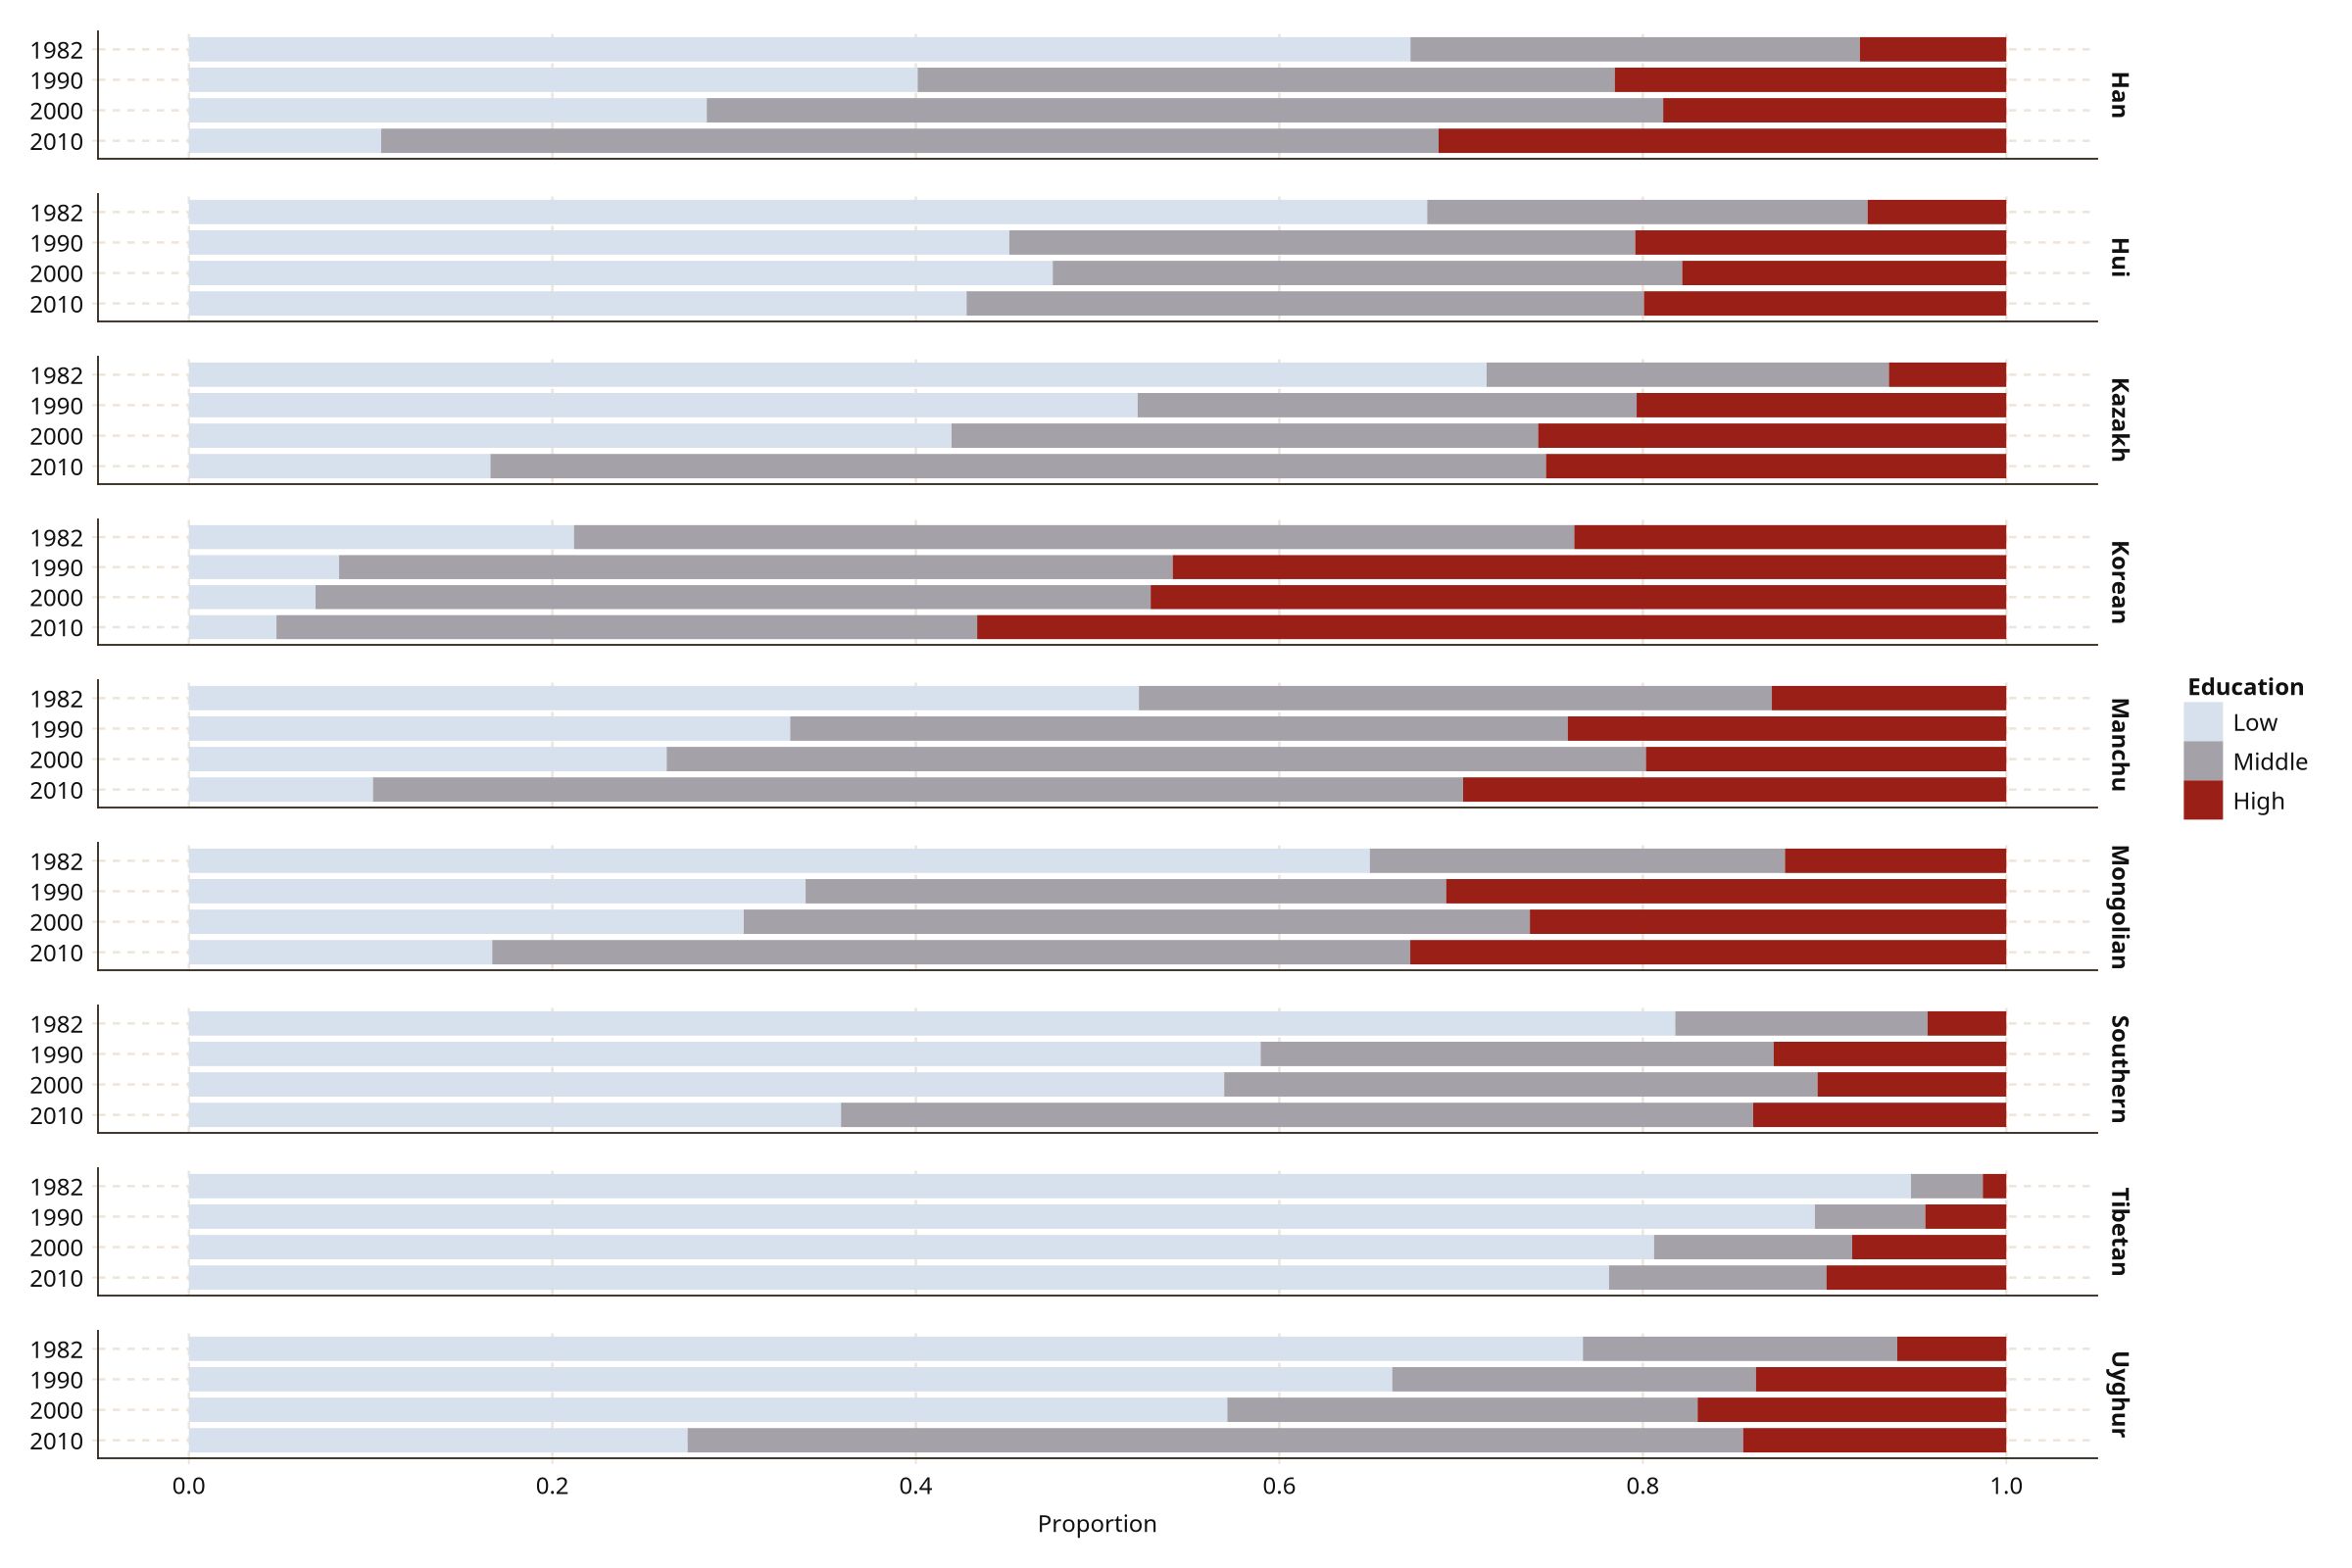
\includegraphics[width=0.7\textwidth]{../graphs/edu_comp.png}
    \caption{Educational composition across ethnic groups, 1982-2010}
    \label{fig:edu_comp}
\end{figure}

When searching for a partner, achieved status (e.g., education) is often considered alongside ascribed status (e.g., ethnicity)
and has gained greater importance during modernization.
We examine how educational compositions have changed across ethnic groups and whether educational advancement facilitates interethnic marriage.

Figure~\ref{fig:edu_comp} illustrates persistent educational disparities across ethnic groups from 1982 to 2010.
Throughout this period, Koreans remained the most educated group,
with 56.63\% of their married population having completed high school in 2010--nearly double the national average of 29.91\%.
The Manchu, Mongolian, and Han populations followed, each with approximately 30\% of their members holding a high school diploma or higher.

At the lower end of the educational spectrum were the Tibetan, Uyghur, and Southern minorities,
with Tibetans experiencing the greatest disadvantage.
Educational expansion had notably less impact on these groups.
For instance, while the national proportion of individuals with primary education or less dropped to 12.85\% by 2010,
among Tibetans this figure remained at 78.14\%, down from 94.75\% in 1982.
Thus, despite overall educational progress, ethnic disparities in educational attainment widened over time

\begin{figure}[htbp]
    \centering
    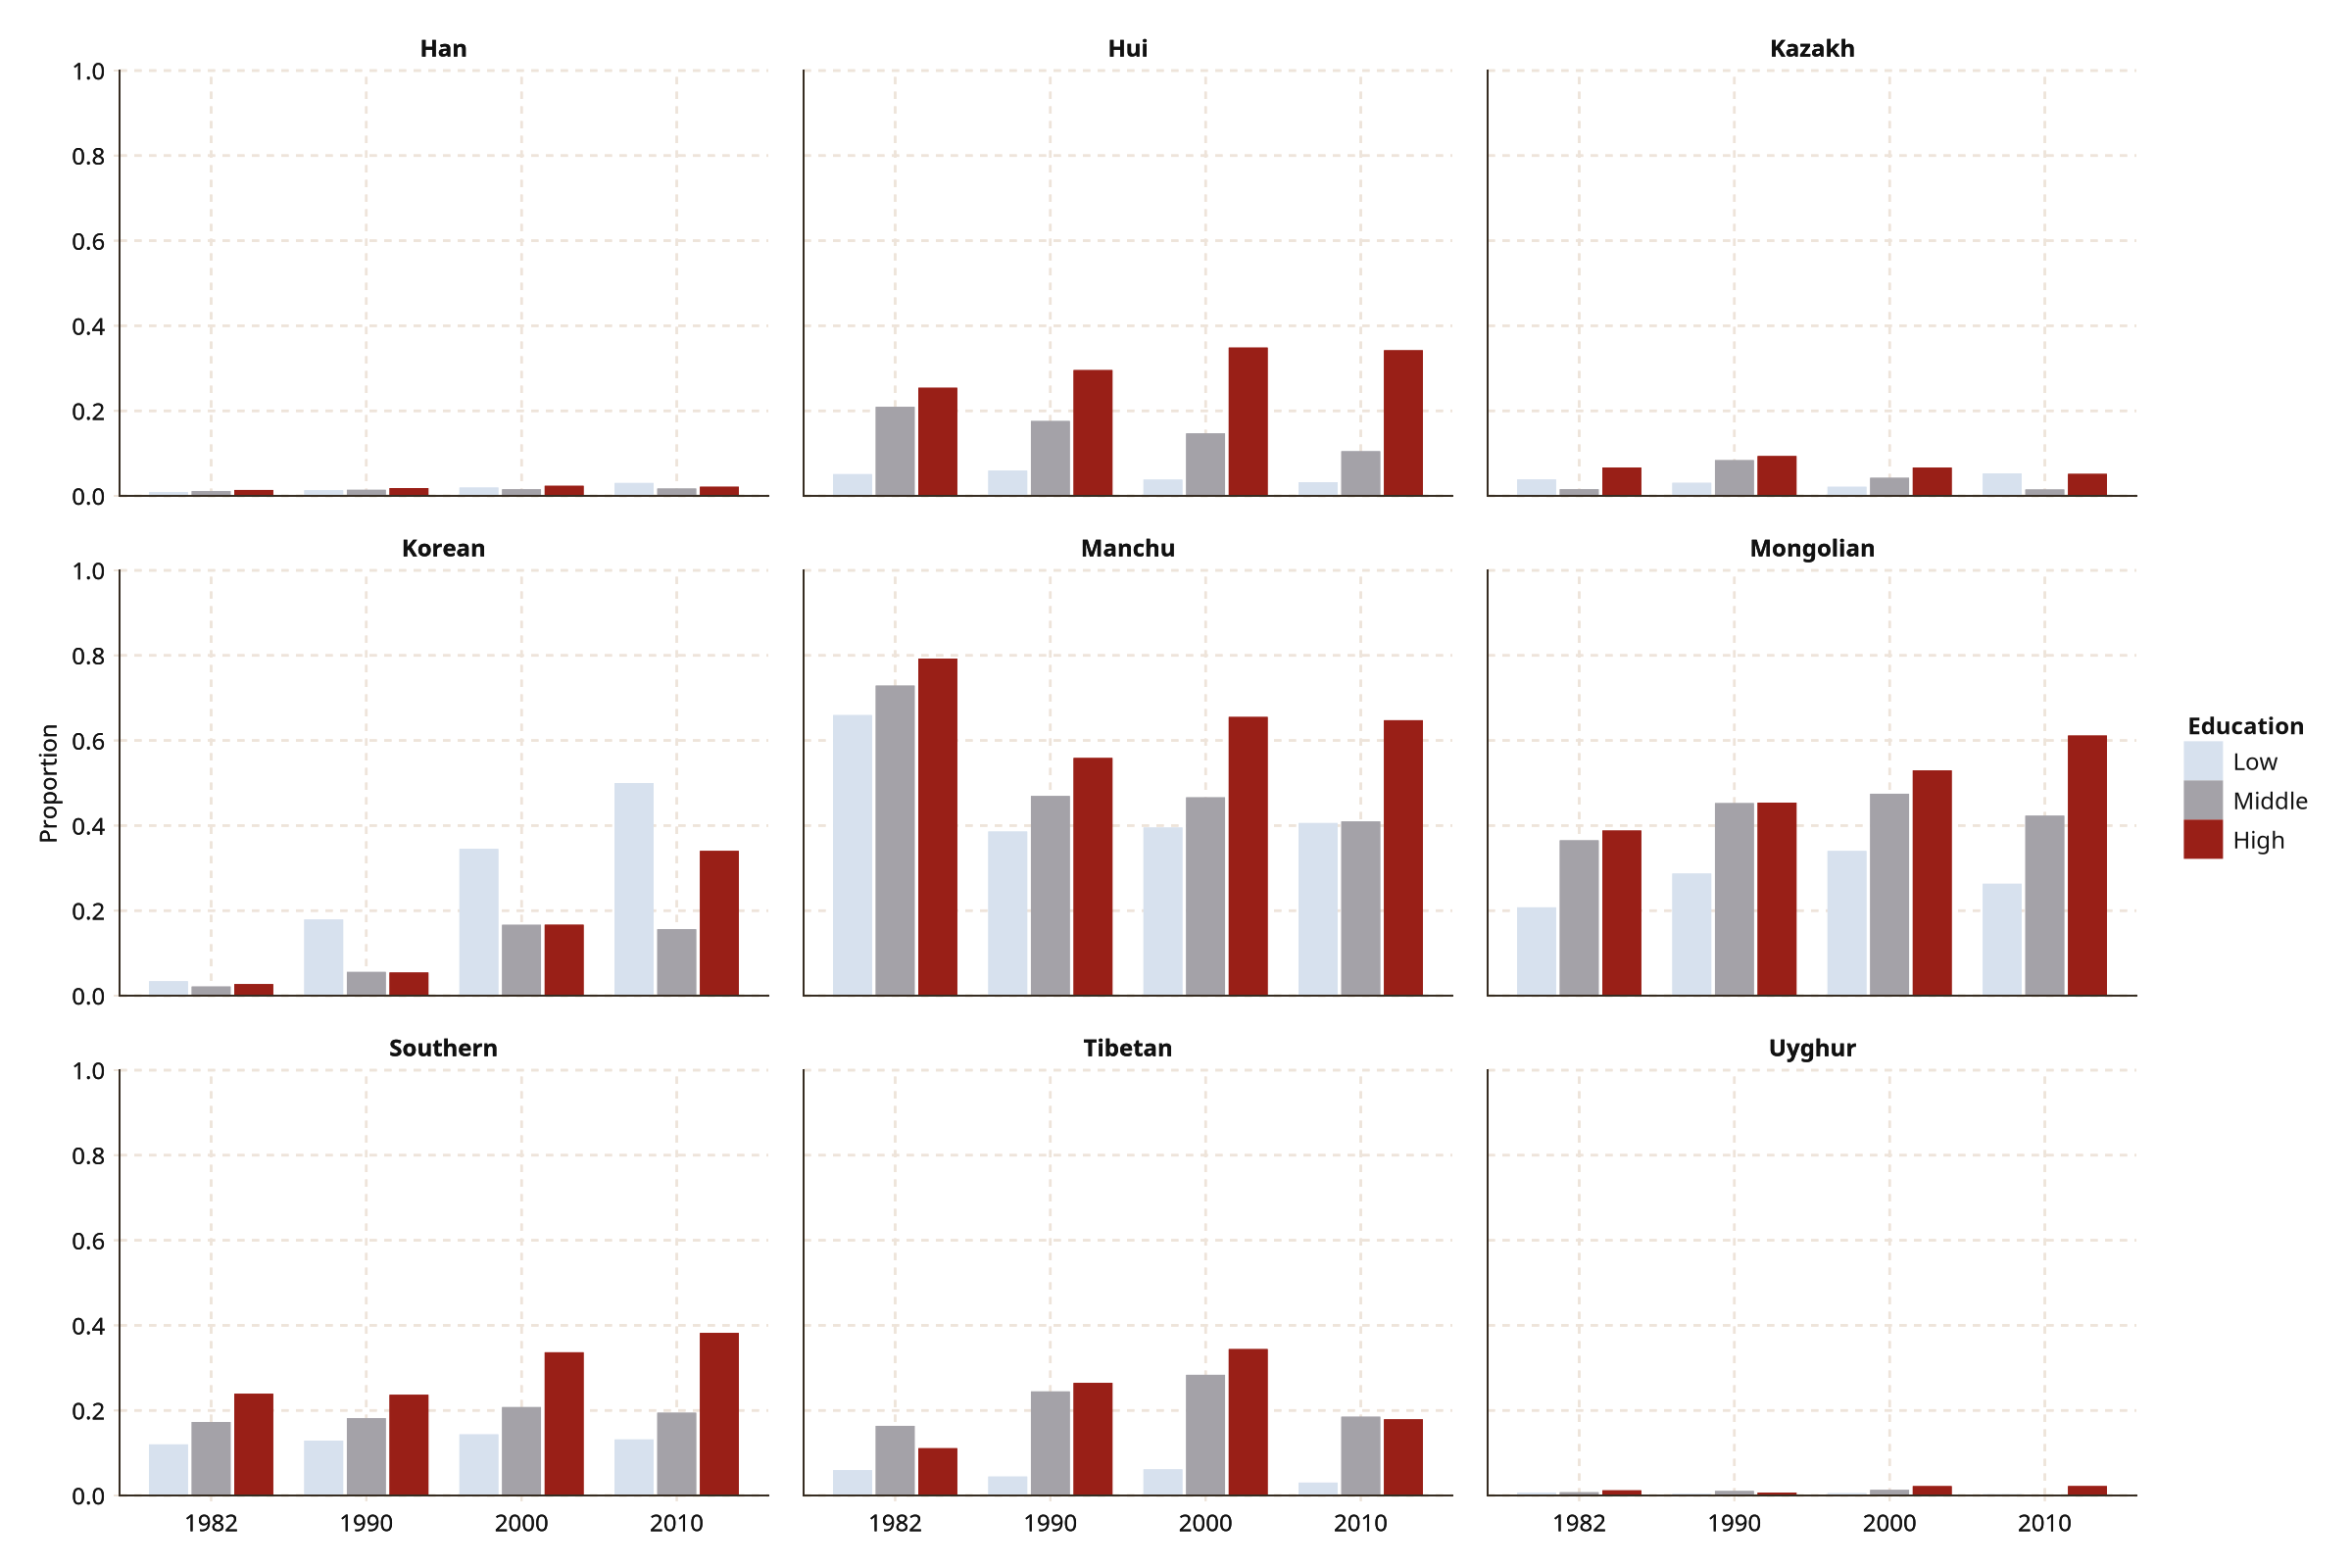
\includegraphics[width=0.7\textwidth]{../graphs/inter_by_edu.png}
    \caption{Proportion of interethnic marriage by educationa and ethnic group, 1982-2010}
    \label{fig:inter_by_edu}
\end{figure}

Figure~\ref{fig:inter_by_edu} illustrates the variation in interethnic marriage rates across educational levels from 1982 to 2010 for each ethnic group.
As shown, there were positive and widening educational gradients in intermarriage rates for the Hui, Manchu, Mongolian, and Southern minorities.
Among the Hui, for example, intermarriage rates in 1982 were 5.11\%, 20.93\%, and 25.42\% for low, middle, and high educational levels, respectively.
By 2010, these rates had shifted to 3.23\%, 10.49\%, and 34.23\%, showing a marked increase in intermarriage among the highly educated.
Similar patterns emerged among the Manchu, Mongolian, and Southern minorities,
where the largest increases--or relatively smaller declines--in intermarriage occurred among those with high school or higher degrees.
The Tibetan population showed less clear educational gradients,
though by 2010, those with middle (18.52\%) or high (17.91\%) school education far exceeded the intermarriage rate of those with low education (3.02\%).

In contrast, the Han majority and Korean populations showed different patterns.
Korean intermarriage rates rose most dramatically among the less educated, from 3.34\% in 1982 to 50\% in 2010,
exceeding the rates for middle (15.63\%) and high (34.04\%) education levels.
Similarly, the Han majority showed higher intermarriage rates
among those with low education (3.04\%) compared to middle (1.73\%) and high (2.15\%) education in 2010.

The Kazakh and Uyghur populations maintained consistently low intermarriage rates across all educational levels.
In 2010, Uyghur intermarriage rates were just 0.29\%, 0.14\%, and 2.21\% for low, middle, and high education levels respectively.

These patterns reveal distinct ethnic differences in how education relates to intermarriage.
While higher education generally corresponds to higher intermarriage rates among the Hui, Manchu, Tibetan, and Southern minorities,
the opposite holds true for Koreans and the Han majority.
The Kazakh and Uyghur populations show minimal intermarriage regardless of education level,
suggesting that ethnic boundaries for these groups remained rigid and largely uninfluenced by instrumental considerations.




\bibliographystyle{apacite}
\bibliography{references}

\clearpage
\appendix
\setcounter{table}{0}
\renewcommand{\thetable}{A\arabic{table}}
\section*{Appendix}

\begin{table}
    \small
    \setlength{\tabcolsep}{4pt}
    \caption{Goodness-of-fit statistics for log-linear models on ethnic pairing}
    \label{tab:goodness-fit1}
    \begin{tabular}{@{}llp{4.5cm}rrrr@{}}
        \hline
        Model                                    & Specification                  &                                                                           & \multicolumn{4}{c}{Goodness-of-fit}                              \\
        \cline{4-7}
                                                 &                                &                                                                           & $G^2$                               & $df$ & ID (\%) & BIC       \\
        \hline
        \multicolumn{3}{@{}l}{Baseline}          &                                &                                                                           &                                     &                            \\
        0                                        & $[T: G_H T: G_W]$              & Conditional independence                                                  & 1,209,960                           & 256  & 10.98   & 1,206,190 \\
        \multicolumn{3}{@{}l}{Ethnic parameters} &                                &                                                                           &                                     &                            \\
        1a                                       & $[T: G_H T: G_W \delta^{HW}]$  & Intra- vs. inter-ethnic marriage                                          & 76,818                              & 255  & 1.74    & 73,026    \\
        1b                                       & $[T: G_H T: G_W \delta^{HW}]$  & Intermarriage with Han vs. minorities                                     & 56,753                              & 254  & 1.44    & 53,011    \\
        1c                                       & $[T: G_H T: G_W \delta^{HW}]$  & Intra-ethnic marriage by ethnicity                                        & 7,028                               & 247  & 0.39    & 3,390     \\
        1d                                       & $[T: G_H T: G_W \delta^{HW}]$  & Inter-ethnic marriage by ethnicity                                        & 6,691                               & 247  & 0.39    & 3,053     \\
        1e                                       & $[T: G_H T: G_W \delta^{HW}]$  & Intra-/inter-ethnic marriage by ethnicity                                 & 4,449                               & 240  & 0.38    & 915       \\
        \multicolumn{3}{@{}l}{Gender parameters} &                                &                                                                           &                                     &                            \\
        2a                                       & $[T: G_H T: G_W \delta^{HW}]$  & Gendered patterns for Hui                                                 & 6,690                               & 246  & 0.39    & 3,067     \\
        2b                                       & $[T: G_H T: G_W \delta^{HW}]$  & Gendered patterns for Kazakh                                              & 6,687                               & 246  & 0.39    & 3,064     \\
        2c                                       & $[T: G_H T: G_W \delta^{HW}]$  & Gendered patterns for Korean                                              & 6,690                               & 246  & 0.39    & 3,067     \\
        2d                                       & $[T: G_H T: G_W \delta^{HW}]$  & Gendered patterns for Manchu                                              & 6,687                               & 246  & 0.39    & 3,064     \\
        2e                                       & $[T: G_H T: G_W \delta^{HW}]$  & Gendered patterns for Mongolian                                           & 6,691                               & 246  & 0.39    & 3,068     \\
        2f                                       & $[T: G_H T: G_W \delta^{HW}]$  & Gendered patterns for Southern                                            & 6,691                               & 246  & 0.39    & 3,068     \\
        2g                                       & $[T: G_H T: G_W \delta^{HW}]$  & Gendered patterns for Tibetan                                             & 6,690                               & 246  & 0.39    & 3,067     \\
        2g                                       & $[T: G_H T: G_W \delta^{HW}]$  & Gendered patterns for Uyghur                                              & 6,691                               & 246  & 0.39    & 3,068     \\
        \multicolumn{3}{@{}l}{Changes over time} &                                &                                                                           &                                     &                            \\
        3a                                       & $[T: G_H T: G_W \delta^{HWT}]$ & Year:Intra- vs. inter-ethnic marriage                                     & 1,534                               & 189  & 0.18    & -1,249    \\
        3b                                       & $[T: G_H T: G_W \delta^{HWT}]$ & \multicolumn{1}{p{4.5cm}}{Year:Intermarriage with Han vs. minorities}     & 1,514                               & 186  & 0.18    & -1,226    \\
        3c                                       & $[T: G_H T: G_W \delta^{HWT}]$ & Year:Intra-ethnic marriage by ethnicity                                   & 200                                 & 165  & 0.01    & -2,230    \\
        3d                                       & $[T: G_H T: G_W \delta^{HWT}]$ & Year:Inter-ethnic marriage by ethnicity                                   & 181                                 & 165  & 0.01    & -2,249    \\
        3e                                       & $[T: G_H T: G_W \delta^{HWT}]$ & \multicolumn{1}{p{4.5cm}}{Year:Intra-/inter-ethnic marriage by ethnicity} & 122                                 & 144  & 0.01    & -1,999    \\
        \multicolumn{3}{@{}l}{Saturated}         &                                &                                                                           &                                     &                            \\
        4                                        & $[T: G_H : G_W]$               &                                                                           & 0                                   & 0    & 0.00    & 0         \\
        \hline
        \multicolumn{7}{@{}p{\textwidth}@{}}{Notes: $G^2$ refers to log-likelihood ratio chi-square statistics, $df$ denotes the degrees of freedom, ID is the index of dissimilarity between observed and predicted numbers, and BIC means the Bayesian information criterion.}
    \end{tabular}
\end{table}

\end{document}